% !TeX spellcheck = en_US
\documentclass[]{report}
\usepackage[english]{babel}

\usepackage[a4paper, margin=0.9in]{geometry}
\usepackage[utf8]{inputenc}
\usepackage{graphicx} 
\usepackage{float}
\usepackage{lscape}
\usepackage[toc,page]{appendix}
\usepackage{subcaption}


\usepackage{listings}
\usepackage{lmodern}  % for bold teletype font
\usepackage{amsmath}  % for \hookrightarrow
\usepackage{xcolor}   % for \textcolor
%\lstloadlanguages{matlab}

\lstset{
	basicstyle=\ttfamily,
	columns=fullflexible,
%	frame=single,
	breaklines=true,
	postbreak=\mbox{\textcolor{red}{$\hookrightarrow$}\space},
}

% Title Page
\title{Simulation of non-central collision}
\author{Dominik Katszer \\Mateusz Nowotyński}

\def\arraystretch{1.5}

\begin{document}
\maketitle

\section{Aim}
The aim of this project is to simulate collision between 2 balls and edges of board.

\section{Model}
\subsection{Body with body collision}
In order to simulate 2d collision(fig. \ref{fig:collision}) we decided to rotate coordinate system to make x axis parallel to contact angle(fig. \ref{fig:collison_rotated}) therefore reducing problem to single dimension. To get speed components in newly created coordinate system we are using equation \ref{eq:rotate_speed}.
\begin{figure}[h]
\begin{subfigure}{.5\textwidth}
	\centering
	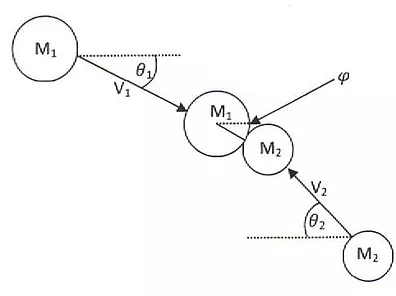
\includegraphics[height=0.8\linewidth]{collision}
	\caption{Draw of simulated collision}
	\label{fig:collision}
\end{subfigure}
\begin{subfigure}{.5\textwidth}
	\centering
	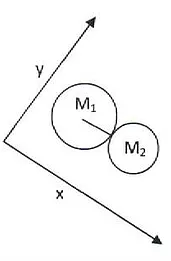
\includegraphics[height=0.8\linewidth]{collision_rotated}
	\caption{Collision with rotated coordinate system}
	\label{fig:collison_rotated}
\end{subfigure}
\caption{}
\end{figure}
\begin{equation}
\begin{aligned}
\label{eq:rotate_speed}
	v_{1xr} &= v_1 cos(\theta_1 - \varphi) \\
	v_{1yr} &= v_1 sin(\theta_1 - \varphi) \\
	v_{2xr} &= v_2 cos(\theta_2 - \varphi) \\
	v_{2yr} &= v_2 sin(\theta_2 - \varphi) 
\end{aligned}
\end{equation}
After that we can calculate as in one dimension case(eq. \ref{eq:single_dim}) since y component is perpendicular to contact angle.
\begin{equation}
\begin{aligned}
\label{eq:single_dim}
v_{1f} &= \frac{v_1(m_1-m_2) + 2m_2v_2}{m_1+m_2} \\
v_{2f} &= \frac{v_2(m_2-m_1) + 2m_1v_1}{m_1+m_2}
\end{aligned}
\end{equation}
And plugging equations \ref{eq:rotate_speed} into \ref{eq:single_dim} we got \ref{eq:roated_x_components}.
\begin{equation}
\begin{aligned}
\label{eq:roated_x_components}
v_{1fxr} &= \frac{v_1 cos(\theta_1 - \varphi)*(m_1-m_2) + 2m_2 v_2 cos(\theta_2 - \varphi)}{m_1+m_2} \\
v_{2fxr} &= \frac{v_2 cos(\theta_2 - \varphi)*(m_2-m_1) + 2m_1 v_1 cos(\theta_1 - \varphi)}{m_1+m_2}
\end{aligned}
\end{equation}
Having speed in rotated coordinate system we can un-rotate it to original one with equation \ref{eq:unrotate_speed},
\begin{equation}
\begin{aligned}
\label{eq:unrotate_speed}
v_{1fx} &= v_{1fxr} cos(\varphi) + v_{1yr} cos(\varphi + \frac{\pi}{2}) \\
v_{1fy} &= v_{1fxr} sin(\varphi) + v_{1yr} sin(\varphi + \frac{\pi}{2}) \\
v_{2fx} &= v_{2fxr} cos(\varphi) + v_{2yr} cos(\varphi + \frac{\pi}{2}) \\
v_{2fy} &= v_{2fxr} sin(\varphi) + v_{2yr} sin(\varphi + \frac{\pi}{2}) 
\end{aligned}
\end{equation}
therefor receiving final equation \ref{eq:final_equation} used to calculate speed after collision in our simulation.
\begin{equation}
\begin{aligned}
\label{eq:final_equation}
v_{1fx} &= \frac{v_1 cos(\theta_1 - \varphi)*(m_1-m_2) + 2m_2 v_2 cos(\theta_2 - \varphi)}{m_1+m_2} cos(\varphi) + v_1 sin(\theta_1 - \varphi) cos(\varphi + \frac{\pi}{2}) \\
v_{1fy} &= \frac{v_1 cos(\theta_1 - \varphi)*(m_1-m_2) + 2m_2 v_2 cos(\theta_2 - \varphi)}{m_1+m_2} sin(\varphi) + v_1 sin(\theta_1 - \varphi) sin(\varphi + \frac{\pi}{2}) \\
v_{2fx} &=\frac{v_2 cos(\theta_2 - \varphi)*(m_2-m_1) + 2m_1 v_1 cos(\theta_1 - \varphi)}{m_1+m_2} cos(\varphi) + v_2 sin(\theta_2 - \varphi) cos(\varphi + \frac{\pi}{2}) \\
v_{2fy} &= \frac{v_2 cos(\theta_2 - \varphi)*(m_2-m_1) + 2m_1 v_1 cos(\theta_1 - \varphi)}{m_1+m_2} sin(\varphi) + v_2 sin(\theta_2 - \varphi) sin(\varphi + \frac{\pi}{2}) 
\end{aligned}
\end{equation}
\subsection{Body with edge collision}
\section{Implementation}
Simulation is implemented in JavaScript using p5js library to render results on canvas. Each ball is moved each frame based on their current velocity,
\begin{lstlisting}
move() {
	this.x = this.x + this.vx;
	this.y = this.y + this.vy;
}
\end{lstlisting}
in every frame we check if two balls intersects with each other
\begin{lstlisting}
intersects(other) {
	let distanceBetweenBalls = dist(this.x, this.y, other.x, other.y);
	return (distanceBetweenBalls < this.r + other.r);
}
\end{lstlisting}
and new velocities are calculated
\begin{lstlisting}
collide(other) {
	let v1 = Math.sqrt(this.vx*this.vx + this.vy*this.vy);
	let v2 = Math.sqrt(other.vx*other.vx + other.vy*other.vy);
	let a1 = this.getAngle();
	let a2 = other.getAngle();
	let ca = this.contactAngle(other);
	let m1 = this.m;
	let m2 = other.m;
	
	let n = v1*Math.cos(a1 - ca)*(m1-m2) + 2 * m2 * v2 * Math.cos(a2 - ca);
	let d = m1 + m2;
	
	
	this.new_vx = n * Math.cos(ca) / d + v1 * Math.sin(a1 - ca) * Math.sin(ca);
	this.new_vy = n * Math.sin(ca) / d + v1 * Math.sin(a1 - ca) * Math.cos(ca);
}
\end{lstlisting}
\section{Conclusion}

\end{document}          
